\documentclass[tikz,border=10pt]{standalone}
\usepackage{tikz}
\usepackage{pgfplots}
\pgfplotsset{compat=1.18}
\usetikzlibrary{arrows.meta, calc}

\begin{document}
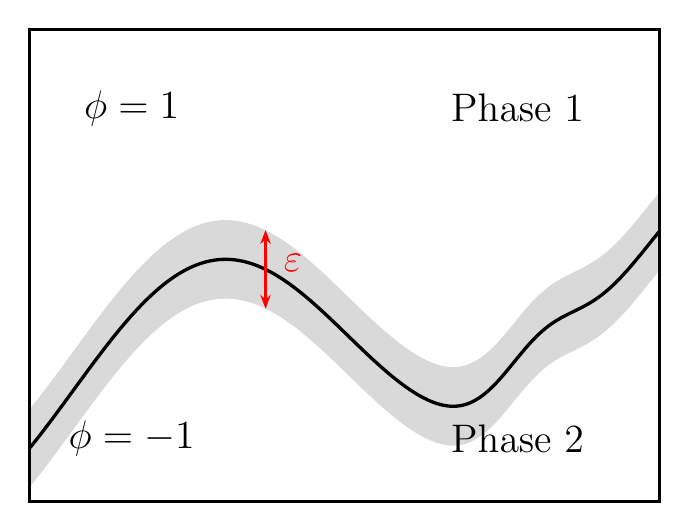
\begin{tikzpicture}

    % --- Dimensions ---
    \def\BoxW{8}
    \def\BoxH{6}
    \def\EpsHalf{0.50}  % half-width of interface band (slightly wider)

    % --- Boundary curve function ---
    % f(x) = 1.5 + 0.25*x + 1.2*sin(0.9*x - 0.5) + 0.6*exp(-((x-6.5)^2)/0.5)
    % Adjusted: reduced slope, increased wave amplitude, added slight right-side correction
    % f(x) = 1.3 + 0.20*x + 1.3*sin(0.9*x - 0.5) + 0.6*exp(-((x-6.5)^2)/0.5)
    \pgfmathdeclarefunction{boundary}{1}{%
        \pgfmathparse{1.3 + 0.20*(#1) + 1.3*sin(0.9*(#1) r - 0.5 r) + 0.6*exp(-((#1)-6.5)*((#1)-6.5)/0.5)}%
    }

    % --- Outer Box (white fill first) ---
    \fill[white] (0,0) rectangle (\BoxW,\BoxH);

    % --- Gray interface band ---
    % Fill gray from upper boundary down to bottom of box
    \fill[gray!30]
        plot[domain=0:\BoxW, samples=200, smooth]
            (\x, {boundary(\x) + \EpsHalf})
        -- (\BoxW, 0) -- (0, 0) -- cycle;

    % Cover below the lower boundary with white
    \fill[white]
        plot[domain=0:\BoxW, samples=200, smooth]
            (\x, {boundary(\x) - \EpsHalf})
        -- (\BoxW, 0) -- (0, 0) -- cycle;

    % Cover above the upper boundary with white
    \fill[white]
        plot[domain=\BoxW:0, samples=200, smooth]
            (\x, {boundary(\x) + \EpsHalf})
        -- (0, \BoxH) -- (\BoxW, \BoxH) -- cycle;

    % --- The main boundary curve (black line) ---
    \draw[black, very thick]
        plot[domain=0:\BoxW, samples=200, smooth]
            (\x, {boundary(\x)});

    % --- Outer box border ---
    \draw[very thick] (0,0) rectangle (\BoxW,\BoxH);

    % --- Labels ---
    % Phase 1 (upper region, phi = 1)
    \node[font=\Large] at (1.3, 5.0) {$\phi = 1$};
    \node[font=\Large] at (6.2, 5.0) {Phase 1};

    % Phase 2 (lower region, phi = -1)
    \node[font=\Large] at (1.3, 0.8) {$\phi = -1$};
    \node[font=\Large] at (6.2, 0.8) {Phase 2};

    % --- Epsilon annotation (red double arrow) ---
    \pgfmathsetmacro{\arrowX}{3.0}
    \pgfmathsetmacro{\fval}{boundary(\arrowX)}
    \pgfmathsetmacro{\arrowBot}{\fval - \EpsHalf}
    \pgfmathsetmacro{\arrowTop}{\fval + \EpsHalf}

    \draw[red, thick, {Stealth[length=5pt]}-{Stealth[length=5pt]}]
        (\arrowX, \arrowBot) -- (\arrowX, \arrowTop);

    \node[red, font=\Large] at ({\arrowX + 0.35}, {\fval + 0.08}) {$\varepsilon$};

\end{tikzpicture}
\end{document}
